\documentclass[a4paper,11pt]{article}

\usepackage{amsmath}
\usepackage[pdftex]{graphicx}

\usepackage[english,greek]{babel}

\usepackage{lmodern}

\usepackage{listings}

\lstset{
  basicstyle=\ttfamily,
  columns=fullflexible,
  frame=single,
  breaklines=true
}

\setlength{\arraycolsep}{2pt}

% Αφαίρεσε (Εισήγαγε) την παρακάτω γραμμή σε σχόλιο αν ο επεξεργαστής κειμένου (δεν) χρησιμοποιεί κωδικοποίηση Unicode για Ελληνικά
\usepackage[utf8x]{inputenc}

% Αφαίρεσε (Εισήγαγε) την παρακάτω γραμμή σε σχόλιο αν ο επεξεργαστής κειμένου (δεν) χρησιμοποιεί κωδικοποίηση iso-8859-7 για Ελληνικά
%\usepackage[iso-8859-7]{inputenc}

%Δημιουργία συντομεύσεων για αλλαγή γραφής σε Ελληνικά/Αγγλικά
\newcommand{\lt}{\latintext}
\newcommand{\gt}{\greektext}

\title{1η Υποχρεωτική Εργασία \\ Στο Μάθημα της Αριθμητικής Ανάλυσης: \\ Άσκηση 4}
\author{Όνοματεπώνυμο: Μπαρακλιλής Ιωάννης  \\  ΑΕΜ: 3685}
\date{18 Δεκεμβρίου 2020}

\begin{document}

\maketitle

\section*{Ζητούμενο 1: Απόδειξη ότι ο πίνακας {\lt G} είναι στοχαστικός}

Πρέπει να αποδείξω ότι ο πίνακας {\lt \textbf{G}} είναι στοχαστικός. Δηλαδη αρκεί να δείξω ότι κάθε στήλη του πίνακα αυτού δίνει άθροισμα 1, δηλαδή να δείξω ότι για κάθε $j$: $\sum_{i=1}^{n} \textbf{{\lt G}}_{(i,j)} = 1$.\\

Έστω \lt $j \in \{1, 2, ..., n\}$,\gt  οπου {\lt n} είναι το πλήθος των στηλών του πίνακα {\lt \textbf{A}}:

\lt

\begin{equation*}
\begin{split}
    \sum_{i=1}^{n} \textbf{G}_{(i,j)} =
    & \sum_{i=1}^{n} \dfrac{q}{n} + \dfrac{\textbf{A}_{(j,i)}(1-q)}{n_j} =
    q\sum_{i=1}^{n} \dfrac{1}{n} + (1-q)\sum_{i=1}^{n} \dfrac{\textbf{A}_{(j,i)}}{n_j} \\
    & = q\cdot 1 + (1 - q)\dfrac{\sum_{i=1}^{n}\textbf{A}_{(j,i)}}{n_j}=
    q + (1 - q)\dfrac{n_j}{n_j} =
    q + 1 - q = 1.
\end{split}
\end{equation*}


\gt Αποδείχθηκε το ζητούμενο.

\section*{Ζητούμενο 2: Εύρεση του πίνακα {\lt G} και του ιδιοδιανύσματος της μέγιστης ιδιοτιμής του}
Ζητείται να κατασκευαστεί ο πίνακας \textbf{\lt G} και να επαληθευτεί με την χρήση της μεθόδου της δυνάμεως ότι το ιδιοδιάνυσμα της μέγιστης ιδιοτιμής είναι αυτό που δίνεται στην εκφώνηση.\\

Αυτά υλοποιούνται προγραμματιστικά στην γλώσσα {\lt python} (3.7) στο αρχείο {\lt b\textunderscore G\textunderscore p\textunderscore calculation.py}  το οποίο φαίνεται παρακάτω:\\


\lt
\lstinputlisting[language=Python]{b_G_p_calculation.py}
\gt

Στον παραπάνω κώδικα:\\
Αρχικά, ορίζεται η συνάρτηση {\lt construct\textunderscore G}, που δέχεται ως παραμέτρους έναν πίνακα Α, έναν πραγματικό αριθμό {\lt q} που αντιστοιχεί στην πιθανότητα μεταπήδησης και έναν ακόμη αριθμό που αντιστοιχεί στο μέγεθος του πίνακα Α, και επιστρέφει τον πίνακα {\lt G} που αντιστοιχεί στις παραμέτρους για τα στοιχεία του οποίου ισχύει ότι {\lt $G_{(i,j)} = \dfrac{q}{n}+\dfrac{A_{(j,i)}(1-q)}{n_j}$} (όπου {\lt $n_j$} είναι το άθροισμα της γραμμής {\lt j}).\\
\par
Στην συνέχεια, ορίζεται η βοηθητική συνάρτηση {\lt matrix\textunderscore columnMatrix\textunderscore multiplication}, που δέχεται ως παραμέτρους έναν πίνακα και έναν πίνακα στήλη (με ίδιο αριθμό γραμμών με τον πίνακα της άλλης παραμέτρου), και επιστρέφει το γινόμενο των δύο πινάκων και η βοηθητική συνάρτηση {\lt integer\textunderscore columnMatrix\textunderscore multiplication}, που δέχεται ως παραμέτρους έναν ακέραιο και έναν πίνακα στήλη, και επιστρέφει τον πίνακα που είναι αποτέλεσμα πολλαπλασιασμού του ακεραίου με τον πίνακα.\\
\par
Ακολούθως ορίζω την συνάρτηση {\lt power\textunderscore method}, που δέχεται ως παραμέτρους έναν πίνακα και τα απαιτούμενα ψηφία ακρίβειας, και επιστέφει το ιδιοδιάνυσμα που αντιστοιχεί στην μέγιστη ιδιοτιμή του πίνακα της παραμέτρου.

\par
Αναλυτικά:\\
Ορίζω (αυθαίρετα) ως (και αποθηκεύω στον πίνακα {\lt p}) αρχική εκτίμηση ιδιοδιανύσματος το ιδιοδιάνυσμα με κάθε του στοιχείο το {\lt $\dfrac{1}{n}$} όπου {\lt n} είναι το πλήθος των στοιχείων του διανύσματος (το άθροισμα των στοιχείων της αρχικής εκτίμησης αυτής του ιδιοδιανύσματος θα είναι 1) και ορίζω την μεταβλητή {\lt eigenvalue\textunderscore estimate} που (θα) αποθηκεύει την εκτίμηση της ιδιοτιμής (την αρχικοποιώ στην τυχαία τιμή 0 που θα αλλάξει στην συνέχεια).\\
Μετά, ξεκινάει ένας ατέρμονος βρόχος που θα τερματίσει όταν <<πετύχω>> ακρίβεια εκτίμησης ιδιοτιμής ίση με αυτή που δόθηκε ως παράμετρος όπου:\\
αποθηκεύω στην (νέα) μεταβλητή {\lt p\textunderscore new} την νέα εκτίμηση του ιδιοδιανύσματος που λαμβάνω πολλαπλασιάζοντας τον πίνακα του ορίσματος με την προηγούμενη εκτίμηση του ιδιοδιανύσματος. Στην συνέχεια, ορίζω την νέα εκτίμηση της ιδιοτιμής (μεταβλητή {\lt new\textunderscore eigenvalue\textunderscore estimate} ως το πρώτο μη μηδενικό στοιχείο της εκτίμησης του ιδιοδιανύσματος (αν δεν έχει μη μηδενικά στοιχεία, δηλαδή είναι το μηδενικό διάνυσμα, τότε η νέα εκτίμηση της ιδιοτιμής θα είναι 0 και σε αυτή την περίπτωση σημαίνει ότι βρέθηκε το ιδιοδιάνυσμα μέγιστης ιδιοτιμής το οποίο είναι η νέα εκτίμηση του ιδιοδιανύσματος που ταυτίζεται με το μηδενικό διάνυσμα την οποία επιστρέφω και τερματίζεται η εκτέλεση της συνάρτησης). Ακολούθως, κανονικοποιώ την νέα εκτίμηση του ιδιοδιανύσματος πολλαπλασιάζοντας κάθε στοιχείο του με το αντίστροφο της ιδιοτιμής. Τελικά, ελέγχω άν η διαφορά της νέας και παλιάς εκτίμησης της ιδιοτιμής είναι μικρότερη απο την ζητούμενη ακρίβεια και αν είναι επιστρέφω την νέα εκτίμηση του ιδιοδιανύσματος μέγιστης ιδιοτιμής. Σε διαφορετική περίπτωση, ενημερώνονται οι μεταβλητές των παλιών εκτιμήσεων ιδιοδιανύσματος και ιδιοτιμής αντίστοιχα.\\

Τέλος ορίζεται η συνάρτηση {\lt main}, χωρίς παραμέτρους, η οποία θα εκτελεστεί όταν θα εκτελέσουμε το παραπάνω αρχείο και εκτελεί τους υπολογισμούς που ζητούνται στην εκφώνηση του ζητούμενου. Αναλυτικά,\\
Αρχικά, ορίζεται ο πίνακας (γειτνίασης του γραφήματος) Α που δίνεται στην εκφώνηση της άσκησης και οι μεταβλητές {\lt q, n} που αντιστοιχούν στην πιθανότητα μεταπήδησης και μέγεθος του πίνακα Α αντίστοιχα. Η μεταβλητή {\lt q} παίρνει την τιμη 0.15 που δίνεται απο την εκφώνηση.\\
Στην συνέχεια, υπολογίζεται και αποθηκεύεται στην μεταβλητή {\lt G} ο πίνακας {\lt Google} που αντιστοιχεί στον πίνακα Α που δημιουργείται με την βοήθεια της συνάρτησης {\lt construct\textunderscore G}.\\
Ακολουθεί εκτύπωση στην οθόνη των στοιχείων (μέχρι 3 δεκαδικά ψηφία) του πίνακα {\lt G} και το άθροισμα κάθε στήλης αυτού, προκειμένου να επαληθευτεί το γεγονός ότι ο {\lt G} είναι στοχαστικός.\\
Μετά, υπολογίζεται και αποθηκεύεται στην μεταβλητή {\lt p\textunderscore result} ο πίνακας με το ιδιοδιάνυσμα που αντιστοιχεί την μέγιστη ιδιοτιμή του {\lt G} (που είναι η 1 εφόσον {\lt G} στοχαστικός) που στην συνέχεια κανονικοποιείται ώστε το άθροισμα των στοιχείων του να δίνει 1.\\
Τελικά, τυπώνονται τα στοιχεία (στρογγυλοποιημένα σε 7 δεκαδικά ψηφία) του ιδιοδιανύσματος μέγιστης ιδιοτιμής του {\lt G} (το οποίο είναι το διάνυσμα με τις τάξεις κάθε σελίδας) και το άθροισμα των στοιχείων του ώστε να επαληθευτεί ότι είναι 1.\\

Άν εκτελέσουμε το αρχείο θα έχουμε ως αποτελέσματα:\\
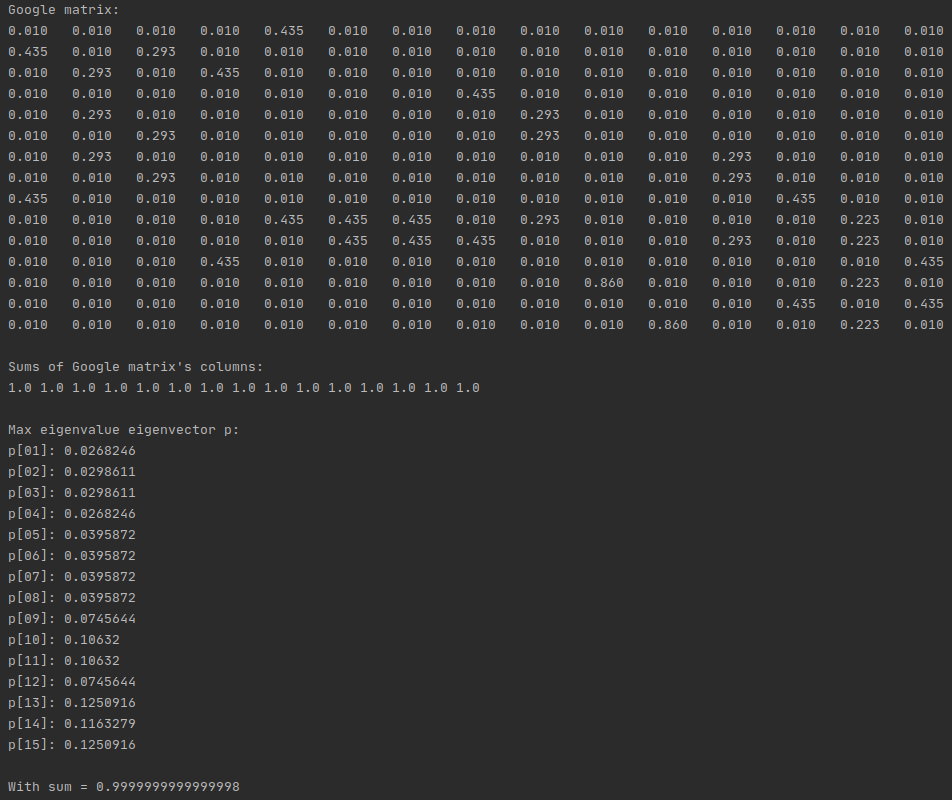
\includegraphics[width=450pt]{Exercise4/run_b.png}\\

Στο παραπάνω μπορούμε να δούμε ότι ο πίνακας {\lt G} (με στοιχεία που εμφανίζονται μέχρι 3 δεκαδικά ψηφία) για το συγκεκριμένο παράδειγμα είναι:\\
\[\textbf{{\lt G}}=
    \left[ \begin{array}{ccccccccccccccc}
    0.010 & 0.010 & 0.010 & 0.010 & 0.435 & 0.010 & 0.010 & 0.010 & 0.010 & 0.010 & 0.010 & 0.010 & 0.010 & 0.010 & 0.010 \\
    0.435 & 0.010 & 0.293 & 0.010 & 0.010 & 0.010 & 0.010 & 0.010 & 0.010 & 0.010 & 0.010 & 0.010 & 0.010 & 0.010 & 0.010 \\
    0.010 & 0.293 & 0.010 & 0.435 & 0.010 & 0.010 & 0.010 & 0.010 & 0.010 & 0.010 & 0.010 & 0.010 & 0.010 & 0.010 & 0.010 \\
    0.010 & 0.010 & 0.010 & 0.010 & 0.010 & 0.010 & 0.010 & 0.435 & 0.010 & 0.010 & 0.010 & 0.010 & 0.010 & 0.010 & 0.010 \\
    0.010 & 0.293 & 0.010 & 0.010 & 0.010 & 0.010 & 0.010 & 0.010 & 0.293 & 0.010 & 0.010 & 0.010 & 0.010 & 0.010 & 0.010 \\
    0.010 & 0.010 & 0.293 & 0.010 & 0.010 & 0.010 & 0.010 & 0.010 & 0.293 & 0.010 & 0.010 & 0.010 & 0.010 & 0.010 & 0.010 \\
    0.010 & 0.293 & 0.010 & 0.010 & 0.010 & 0.010 & 0.010 & 0.010 & 0.010 & 0.010 & 0.010 & 0.293 & 0.010 & 0.010 & 0.010 \\
    0.010 & 0.010 & 0.293 & 0.010 & 0.010 & 0.010 & 0.010 & 0.010 & 0.010 & 0.010 & 0.010 & 0.293 & 0.010 & 0.010 & 0.010 \\
    0.435 & 0.010 & 0.010 & 0.010 & 0.010 & 0.010 & 0.010 & 0.010 & 0.010 & 0.010 & 0.010 & 0.010 & 0.435 & 0.010 & 0.010 \\
    0.010 & 0.010 & 0.010 & 0.010 & 0.435 & 0.435 & 0.435 & 0.010 & 0.293 & 0.010 & 0.010 & 0.010 & 0.010 & 0.223 & 0.010 \\
    0.010 & 0.010 & 0.010 & 0.010 & 0.010 & 0.435 & 0.435 & 0.435 & 0.010 & 0.010 & 0.010 & 0.293 & 0.010 & 0.223 & 0.010 \\
    0.010 & 0.010 & 0.010 & 0.435 & 0.010 & 0.010 & 0.010 & 0.010 & 0.010 & 0.010 & 0.010 & 0.010 & 0.010 & 0.010 & 0.435 \\
    0.010 & 0.010 & 0.010 & 0.010 & 0.010 & 0.010 & 0.010 & 0.010 & 0.010 & 0.860 & 0.010 & 0.010 & 0.010 & 0.223 & 0.010 \\
    0.010 & 0.010 & 0.010 & 0.010 & 0.010 & 0.010 & 0.010 & 0.010 & 0.010 & 0.010 & 0.010 & 0.010 & 0.435 & 0.010 & 0.435 \\
    0.010 & 0.010 & 0.010 & 0.010 & 0.010 & 0.010 & 0.010 & 0.010 & 0.010 & 0.010 & 0.860 & 0.010 & 0.010 & 0.223 & 0.010
    \end{array} \right]
\]
όπου κάθε στήλη του έχει άθροισμα 1 (επαληθεύοντας το ζητούμενο 1 ότι ο πίνακας {\lt G} είναι στοχαστικός)\\

Επίσης, βλέπουμε ότι το ιδιοδιάνυσμα που αντιστοιχεί στην μέγιστη ιδιοτιμή είναι:\\
\[\textbf{{\lt p}}=
    \left[ \begin{array}{c}
    0.0268246 \\
    0.0298611 \\
    0.0298611 \\
    0.0268246 \\
    0.0395872 \\
    0.0395872 \\
    0.0395872 \\
    0.0395872 \\
    0.0745644 \\
    0.10632 \\
    0.10632 \\
    0.0745644 \\
    0.1250916 \\
    0.1163279 \\
    0.1250916 \\
    \end{array} \right]
\]
που έχει σφάλμα σε σχέση με αυτό της εκφώνησης (ως προς την μέγιστη νόρμα) $\simeq 0.26392 \cdot 10 ^ -7$.

\section*{Ζητούμενο 3: Βελτίωση σημαντικότητας επιλεγμένης σελίδας με ορισμένες αλλαγές στις συνδέσεις}
Ζητείται να προστεθούν 4 συνδέσεις και να αφαιρεθεί 1 από αυτές που ήδη υπάρχουν στο γράφημα και να κατασκευαστεί ο νέος πίνακα {\lt G} έτσι ώστε να βελτιωθεί ο βαθμός σημαντικότητας μιας σελίδας που θα επιλέξω.\\

\par
Επιλέγω να βελτιώσω την τάξη της σελίδας 1.\\
Απο την εκφώνηση της άσκησης γνωρίζουμε ότι η σημαντικότητα μία σελίδας δεν κρίνεται αυστηρά και μόνο απο τον αριθμό των σελιδών που <<δείχνουν>> σε αυτή αλλά λαμβάνεται υπόψιν και το γεγονός ότι όταν μία σελίδα <<δείχνει>> σε μία άλλη <<μεταφέρει>> κάποια απο την σημαντικότητα της. Επομένως, με την προσθήκη και αφαίρεση συνδέσεων, στόχος μου είναι να μεγιστοποιήσω την <<μεταφορά>> σημαντικότητας πρός και να ελαχιστοποιήσω την μεταφορά σημαντικότητας από την σελίδα 1. \\
Τέλος, αξίζει να σημειωθεί ότι η σημαντικότητα <<πηγάζει>> απο τον αριθμό εισερχόμενων συνδέσεων ακόμη και αν δεν βασίζεται αποκλειστικά σε αυτόν. Δηλαδή, η σελίδα 13 έχει μεγάλη σημαντικότητα λόγω της άμεσης και έμεσης σύνδεσης της με τις σελίδες 10 και 11 που έχουν μεγάλο αριθμό εισερχόμενων συνδέσεων. Αν για παράδειγμα η σελίδα 10 σταματήσει να <<δείχνει>> στην 13, αυτή χάνει σημαντικότητα. Ομοίως, αν η 10 αρχίσει να δείχνει σε κάποια άλλη σελίδα εκτός της 13, το <<ποσό>> σημαντικότητας που θα μεταφερθεί στην 13 μειώνεται γιατί το <<ποσό>> σημαντικότητας που μεταφέρεται απο την σελίδα 10 εξαρτάται απο τον αριθμό των σελιδών στις οποίες δείχνει η σελίδα 10.\\

\par
Επομένως, λαμβάνοντας υπόψιν τις παραπάνω παρατηρήσεις:\\
Αρχικά, προσθέτω συνδέσεις απο την 10 στην 1 και απο την 11 στην 1, έτσι <<μεταφέρεται>> (κάποια απο την) σημαντικότητα αυτών προς την 1.\\
Στην συνέχεια, προσθέτω συνδέσεις απο την 15 στην 1, ώστε να <<μεταφέρεται>> κάποια απο την σημαντικότητα που <<πηγαίνει>> απο την 11 στην 15 να <<πηγαίνει>> στην 1, και απο την 2 στην 1, ώστε η σημαντικότητα που <<φεύγει>> απο την 1 προς στην 2 να <<επιστρέφει στην 1>>.
Τέλος, αφαιρώ την σύνδεση απο την 10 στην 13, ώστε όλη η <<μεταφορά>> σημαντικότητας να γίνεται αποκλειστικά προς την 1.\\

Επομένως καταλήγουμε με έναν πίνακα γειτνίασης της μορφής:\\

\[\textbf{{\lt A}}=
    \left[ \begin{array}{ccccccccccccccc}
    0 & 1 & 0 & 0 & 0 & 0 & 0 & 0 & 1 & 0 & 0 & 0 & 0 & 0 & 0 \\
    1 & 0 & 1 & 0 & 1 & 0 & 1 & 0 & 0 & 0 & 0 & 0 & 0 & 0 & 0 \\
    0 & 1 & 0 & 0 & 0 & 1 & 0 & 1 & 0 & 0 & 0 & 0 & 0 & 0 & 0 \\
    0 & 0 & 1 & 0 & 0 & 0 & 0 & 0 & 0 & 0 & 0 & 1 & 0 & 0 & 0 \\
    1 & 0 & 0 & 0 & 0 & 0 & 0 & 0 & 0 & 1 & 0 & 0 & 0 & 0 & 0 \\
    0 & 0 & 0 & 0 & 0 & 0 & 0 & 0 & 0 & 1 & 1 & 0 & 0 & 0 & 0 \\
    0 & 0 & 0 & 0 & 0 & 0 & 0 & 0 & 0 & 1 & 1 & 0 & 0 & 0 & 0 \\
    0 & 0 & 0 & 1 & 0 & 0 & 0 & 0 & 0 & 0 & 1 & 0 & 0 & 0 & 0 \\
    0 & 0 & 0 & 0 & 1 & 1 & 0 & 0 & 0 & 1 & 0 & 0 & 0 & 0 & 0 \\
    1 & 0 & 0 & 0 & 0 & 0 & 0 & 0 & 0 & 0 & 0 & 0 & 0 & 0 & 0 \\
    1 & 0 & 0 & 0 & 0 & 0 & 0 & 0 & 0 & 0 & 0 & 0 & 0 & 0 & 1 \\
    0 & 0 & 0 & 0 & 0 & 0 & 1 & 1 & 0 & 0 & 1 & 0 & 0 & 0 & 0 \\
    0 & 0 & 0 & 0 & 0 & 0 & 0 & 0 & 1 & 0 & 0 & 0 & 0 & 1 & 0 \\
    0 & 0 & 0 & 0 & 0 & 0 & 0 & 0 & 0 & 1 & 1 & 0 & 1 & 0 & 1 \\
    1 & 0 & 0 & 0 & 0 & 0 & 0 & 0 & 0 & 0 & 0 & 1 & 0 & 1 & 0
    \end{array} \right]
\]


Προγραμματιστικά, η κατασκευή νέου πίνακα {\lt G} και ο υπολογισμός νέας τάξης σελιδών γίνεται στην γλώσσα {\lt python} στο αρχείο {\lt c\textunderscore Graph\textunderscore Modifications.py} το οποίο φαίνεται παρακάτω:\\

\lt
\lstinputlisting[language=Python]{c_Graph_Modifications.py}
\gt

Στον παραπάνω κώδικα:\\
Αρχικά, ορίζονται εκ νέου οι  συναρτήσεις {\lt construct\textunderscore G}, {\lt matrix\textunderscore columnMatrix\textunderscore multiplication}, {\lt integer\textunderscore columnMatrix\textunderscore multiplication} και {\lt power\textunderscore method} του αρχείου {\lt b\textunderscore G\textunderscore p\textunderscore calculation.py} που βρίσκεται στον ίδιο φάκελο {\lt Exercise4} μαζί με το τρέχον.
Αμέσως μετά βρίσκεται ο εκτελέσιμος κώδικας που θα εκτελεστεί αν εκτελέσουμε το αρχείο:\\
Ορίζεται ο νέος πίνακας (γειτνίασης του γραφήματος) Α (σύμφωνα με τα παραπάνω). Στην συνέχεια, κατασκευάζεται ο πίνακας {\lt G} και τυπώνονται τα στοιχεία του και το άθροισμα των στηλών του (για επαλήθευση ότι είναι στοχαστικός). Στην συνέχεια, υπολογίζεται το ιδιοδιάνυσμα της μέγιστης ιδιοτιμής (που είναι η 1 εφόσον ο {\lt G} είναι στοχαστικός) και αφού κανονικοποιηθεί αποτελεί τον πίνακα με τις τάξεις των σελίδων. Τέλος εμφανίζονται στην οθόνη οι τάξεις των σελίδων (στρογγυλοποιημένες σε 7 δεκαδικά ψηφία) και το άθροισμα όλων των τάξεων (για επαλήθευση ότι αθροίζουν στο 1 ως πιθανότητες).\\

Άν εκτελέσουμε το αρχείο έχουμε:\\
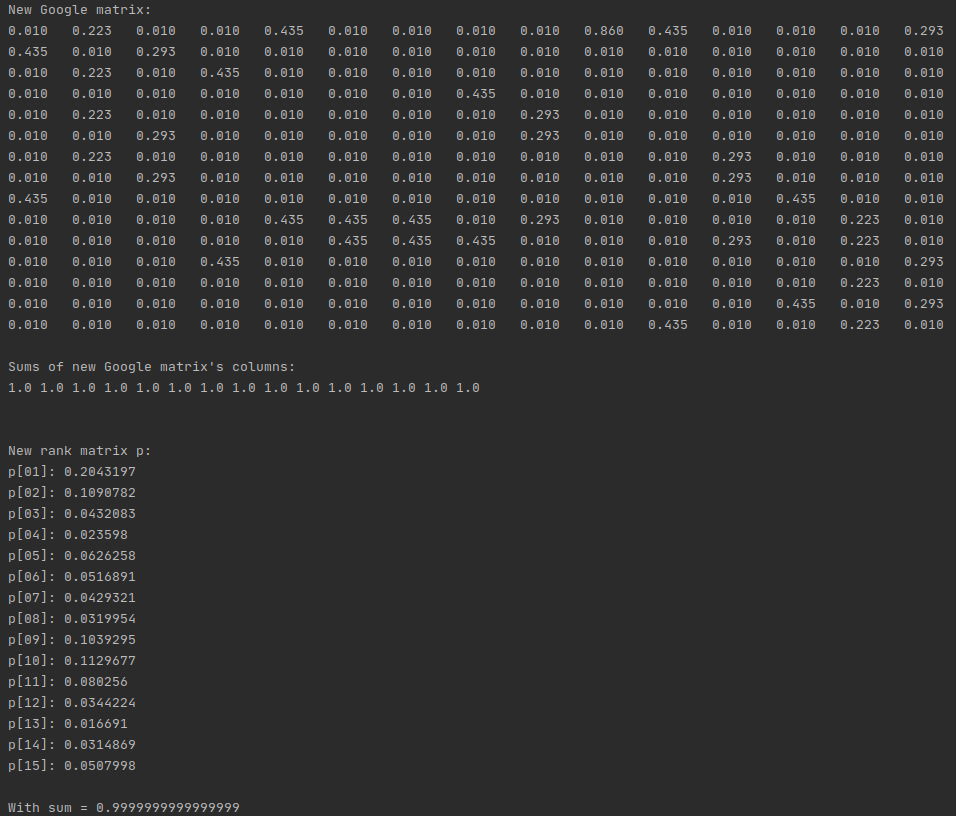
\includegraphics[width=450pt]{Exercise4/run_c.png}\\

Στο παραπάνω μπορούμε να δούμε ότι ο νέος πίνακας {\lt G} είναι:\\
\[\textbf{{\lt G}}=
    \left[ \begin{array}{ccccccccccccccc}
    0.010 & 0.223 & 0.010 & 0.010 & 0.435 & 0.010 & 0.010 & 0.010 & 0.010 & 0.860 & 0.435 & 0.010 & 0.010 & 0.010 & 0.293 \\
    0.435 & 0.010 & 0.293 & 0.010 & 0.010 & 0.010 & 0.010 & 0.010 & 0.010 & 0.010 & 0.010 & 0.010 & 0.010 & 0.010 & 0.010 \\
    0.010 & 0.223 & 0.010 & 0.435 & 0.010 & 0.010 & 0.010 & 0.010 & 0.010 & 0.010 & 0.010 & 0.010 & 0.010 & 0.010 & 0.010 \\
    0.010 & 0.010 & 0.010 & 0.010 & 0.010 & 0.010 & 0.010 & 0.435 & 0.010 & 0.010 & 0.010 & 0.010 & 0.010 & 0.010 & 0.010 \\
    0.010 & 0.223 & 0.010 & 0.010 & 0.010 & 0.010 & 0.010 & 0.010 & 0.293 & 0.010 & 0.010 & 0.010 & 0.010 & 0.010 & 0.010 \\
    0.010 & 0.010 & 0.293 & 0.010 & 0.010 & 0.010 & 0.010 & 0.010 & 0.293 & 0.010 & 0.010 & 0.010 & 0.010 & 0.010 & 0.010 \\
    0.010 & 0.223 & 0.010 & 0.010 & 0.010 & 0.010 & 0.010 & 0.010 & 0.010 & 0.010 & 0.010 & 0.293 & 0.010 & 0.010 & 0.010 \\
    0.010 & 0.010 & 0.293 & 0.010 & 0.010 & 0.010 & 0.010 & 0.010 & 0.010 & 0.010 & 0.010 & 0.293 & 0.010 & 0.010 & 0.010 \\
    0.435 & 0.010 & 0.010 & 0.010 & 0.010 & 0.010 & 0.010 & 0.010 & 0.010 & 0.010 & 0.010 & 0.010 & 0.435 & 0.010 & 0.010 \\
    0.010 & 0.010 & 0.010 & 0.010 & 0.435 & 0.435 & 0.435 & 0.010 & 0.293 & 0.010 & 0.010 & 0.010 & 0.010 & 0.223 & 0.010 \\
    0.010 & 0.010 & 0.010 & 0.010 & 0.010 & 0.435 & 0.435 & 0.435 & 0.010 & 0.010 & 0.010 & 0.293 & 0.010 & 0.223 & 0.010 \\
    0.010 & 0.010 & 0.010 & 0.435 & 0.010 & 0.010 & 0.010 & 0.010 & 0.010 & 0.010 & 0.010 & 0.010 & 0.010 & 0.010 & 0.293 \\
    0.010 & 0.010 & 0.010 & 0.010 & 0.010 & 0.010 & 0.010 & 0.010 & 0.010 & 0.010 & 0.010 & 0.010 & 0.010 & 0.223 & 0.010 \\
    0.010 & 0.010 & 0.010 & 0.010 & 0.010 & 0.010 & 0.010 & 0.010 & 0.010 & 0.010 & 0.010 & 0.010 & 0.435 & 0.010 & 0.293 \\
    0.010 & 0.010 & 0.010 & 0.010 & 0.010 & 0.010 & 0.010 & 0.010 & 0.010 & 0.010 & 0.435 & 0.010 & 0.010 & 0.223 & 0.010 \\
    \end{array} \right]
\]
όπου κάθε στήλη του έχει άθροισμα 1 (επαληθεύοντας το ζητούμενο 1 ότι ο πίνακας {\lt G} είναι στοχαστικός)\\

Επίσης, βλέπουμε ότι το διάνυσμα με τις τάξεις των σελίδων είναι:\\
\[\textbf{{\lt p}}=
    \left[ \begin{array}{c}
    0.2043197 \\
    0.1090782 \\
    0.0432083 \\
    0.023598 \\
    0.0626258 \\
    0.0516891 \\
    0.0429321 \\
    0.0319954 \\
    0.1039295 \\
    0.1129677 \\
    0.080256 \\
    0.0344224 \\
    0.016691 \\
    0.0314869 \\
    0.0507998 \\
    \end{array} \right]
\]

Επομένως, βλέπουμε ότι η τάξη της σελίδας 1 (1ο στοιχείο του διανύσματος με τις τάξεις) είναι 0.2043197 σε σχέση με 0.0268246 που ήταν πρίν τις μεταβολές (απο ζητούμενο 2).\\
Βλέπουμε μία αύξηση $0.2043197 - 0.0268246 = 0.1774951$.

\section*{Ζητούμενο 4: Αλλαγή και μελέτη της πιθανότητα μεταπήδησης {\lt q} στον νέο γράφο}
Ζητείται να γίνει αλλαγή της πιθανότητας μεταπήδησης {\lt q} σε (α) {\lt q} = 0.02 και (β) {\lt q} = 0.6 στον νέο γράφο και να γίνει περιγραφή των αλλαγών στην τάξη σελίδας.\\

Αυτά υλοποιούνται προγραμματιστικά στην γλώσσα {\lt python} στο αρχείο {\lt d\textunderscore p\textunderscore Modifications.py}  το οποίο φαίνεται παρακάτω:\\


\lt
\lstinputlisting[language=Python]{d_p_Modifications.py}
\gt

Στον παραπάνω κώδικα:\\
Αρχικά, ορίζονται εκ νέου οι  συναρτήσεις {\lt construct\textunderscore G}, {\lt matrix\textunderscore columnMatrix\textunderscore multiplication}, {\lt integer\textunderscore columnMatrix\textunderscore multiplication} και {\lt power\textunderscore method} του αρχείου {\lt b\textunderscore G\textunderscore p\textunderscore calculation.py} που βρίσκεται στον ίδιο φάκελο {\lt Exercise4} μαζί με το τρέχον.
Αμέσως μετά βρίσκεται ο εκτελέσιμος κώδικας που θα εκτελεστεί αν εκτελέσουμε το αρχείο:\\
Ορίζεται ο πίνακας (γειτνίασης του γραφήματος) Α που είναι πανομοιότυπος με εκείνον του προηγούμενου ζητούμενου (ζητούμενο 3).\\
Μετά, για κάθε ένα απο τα {\lt q} ({\lt q = 0.02} και {\lt q = 0.6}): ορίζεται η μεταβλητή {\lt q} που αποθηκεύει την πιθανότητας μεταπήδησης και η μεταβλητή {\lt n} που αποθηκεύει το μέγεθος του πίνακα Α. Στην συνέχεια, κατασκευάζεται ο πίνακας {\lt G}. Στην συνέχεια, υπολογίζεται το ιδιοδιάνυσμα της μέγιστης ιδιοτιμής και αφού κανονικοποιηθεί αποτελεί τον πίνακα με τις τάξεις των σελίδων. Τέλος εμφανίζονται στην οθόνη οι τάξεις των σελίδων (στρογγυλοποιημένες σε 7 δεκαδικά ψηφία) και το άθροισμα όλων των τάξεων (για επαλήθευση ότι αθροίζουν στο 1 ως πιθανότητες).\\

Άν εκτελέσουμε το αρχείο αυτό το αρχείο θα δούμε στην οθόνη:\\
\begin{center}
    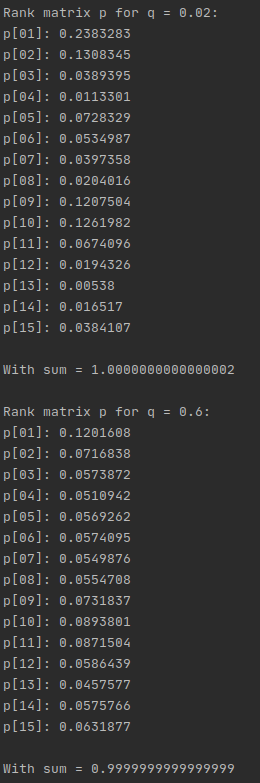
\includegraphics[width=150pt]{Exercise4/run_d.png}\\
\end{center}

Για {\lt q = 0.02} έχουμε διάνυσμα με τις τάξεις των σελίδων:\\
\[\textbf{{\lt p}}=
    \left[ \begin{array}{c}
    0.2383283 \\
    0.1308345 \\
    0.0389395 \\
    0.0113301 \\
    0.0728329 \\
    0.0534987 \\
    0.0397358 \\
    0.0204016 \\
    0.1207504 \\
    0.1261982 \\
    0.0674096 \\
    0.0194326 \\
    0.00538 \\
    0.016517 \\
    0.0384107 \\
    \end{array} \right]
\]

Συμπεραίνουμε ότι αύξηση έχουν οι σελίδες 1, 2, 5, 6, 9, 10 και μείωση οι υπόλοιπες.\\
Παρατηρούμε ότι οι σελίδες με μεγάλη (πριν την αλλαγή) τάξη, όπως 1, 2, 9, 10 αυξάνουν την τάξη τους. Παράλληλα, μερικές σελίδες που συνδέονται άμεσα με τις παραπάνω που είναι οι 5 και 6, βλέπουν επίσης βελτίωση στην τάξη τους. Τέλος, άλλες σελίδες που δεν συνδέονται άμεσα με αυτές με μεγάλη (πριν την αλλαγή) τάξη έχουν μείωση της τάξης τους.\\

Επίσης, για {\lt q = 0.6} έχουμε διάνυσμα με τις τάξεις των σελίδων:\\
\[\textbf{{\lt p}}=
    \left[ \begin{array}{c}
    0.1201608 \\
    0.0716838 \\
    0.0573872 \\
    0.0510942 \\
    0.0569262 \\
    0.0574095 \\
    0.0549876 \\
    0.0554708 \\
    0.0731837 \\
    0.0893801 \\
    0.0871504 \\
    0.0586439 \\
    0.0457577 \\
    0.0575766 \\
    0.0631877 \\
    \end{array} \right]
\]

Συμπεραίνουμε ότι μείωση έχουν οι σελίδες 1, 2, 5, 9, 10 και αύξηση οι υπόλοιπες.\\
Παρατηρούμε ότι οι σελίδες με μεγάλη (πριν την αλλαγή) τάξη, όπως 1, 2, 9, 10 μειώνουν την τάξη τους. Παράλληλα, μία σελίδα που συνδέεται άμεσα με τις παραπάνω που είναι η 5, βλέπει επίσης μείωση στην τάξη της. Τέλος, άλλες σελίδες που δεν συνδέονται άμεσα με αυτές με μεγάλη (πριν την αλλαγή) τάξη έχουν αύξηση της τάξης τους.\\

\par
Τέλος, σχετικά με την πιθανότητα μεταπήδησης, αυτή ορίζει την πιθανότητα να βρεθεί ο χρήστης σε οποιαδήποτε σελίδα του γραφήματος ανεξαρτήτως της διασύνδεσης αυτών. Επομένως, δίνει μία <<βασική>> πιθανότητα να βρεθεί ο χρήστης σε κάποια σελίδα η οποία μετά μεταβάλλεται ανάλογα με τις διασυνδέσεις και έτσι <<ρυθμίζει>> την σημασία των διασυνδέσεων στην τάξη της σελίδας.\\
Το παραπάνω επαληθεύεται, αν δούμε τα αποτελέσματα της εκτέλεσης του κώδικα αυτού του ζητουμένου: Όταν μειώνουμε το {\lt q} απο 0.15 σε 0.02 βλέπουμε ότι οι σελίδες στις οποίες συνδέονται πολλές σελίδες άμεσα ή λιγότερο άμεσα βλέπουν αύξηση της τάξης τους ενώ, σελίδες στις οποίες δεν συνδέονται πολλές άλλες βλέπουν μείωση. Αντίστοιχα, όταν αυξάνουμε το {\lt q} απο 0.15 σε 0.6 παρατηρούμε το αντίθετο φαινόμενο.

\section*{Ζητούμενο 5: Απόπειρα βελτίωσης της σελίδας 11}
Ζητείται να μελετηθεί η απόπειρα της σελίδας 11 του αρχικού γραφήματος να βελτιώσει την σχέση της με τον ανταγωνιστή της όταν το αποτέλεσμα των προσπαθειών της μοντελοποιείται με το να έχουμε τον αρχικό πίνακα (γειτνίασης του γραφήματος) Α για τον οποίο όμως ισχύει ότι {\lt $\textbf{A}_{(8, 11)} = \textbf{A}_{(12, 11)} = 3$}.\\

Επομένως έχουμε τον τροποποιημένο πίνακα γειτνίασης Α:
\[\textbf{{\lt A}}=
    \left[ \begin{array}{ccccccccccccccc}
    0 & 1 & 0 & 0 & 0 & 0 & 0 & 0 & 1 & 0 & 0 & 0 & 0 & 0 & 0 \\
    0 & 0 & 1 & 0 & 1 & 0 & 1 & 0 & 0 & 0 & 0 & 0 & 0 & 0 & 0 \\
    0 & 1 & 0 & 0 & 0 & 1 & 0 & 1 & 0 & 0 & 0 & 0 & 0 & 0 & 0 \\
    0 & 0 & 1 & 0 & 0 & 0 & 0 & 0 & 0 & 0 & 0 & 1 & 0 & 0 & 0 \\
    1 & 0 & 0 & 0 & 0 & 0 & 0 & 0 & 0 & 1 & 0 & 0 & 0 & 0 & 0 \\
    0 & 0 & 0 & 0 & 0 & 0 & 0 & 0 & 0 & 1 & 1 & 0 & 0 & 0 & 0 \\
    0 & 0 & 0 & 0 & 0 & 0 & 0 & 0 & 0 & 1 & 1 & 0 & 0 & 0 & 0 \\
    0 & 0 & 0 & 1 & 0 & 0 & 0 & 0 & 0 & 0 & 3 & 0 & 0 & 0 & 0 \\
    0 & 0 & 0 & 0 & 1 & 1 & 0 & 0 & 0 & 1 & 0 & 0 & 0 & 0 & 0 \\
    0 & 0 & 0 & 0 & 0 & 0 & 0 & 0 & 0 & 0 & 0 & 0 & 1 & 0 & 0 \\
    0 & 0 & 0 & 0 & 0 & 0 & 0 & 0 & 0 & 0 & 0 & 0 & 0 & 0 & 1 \\
    0 & 0 & 0 & 0 & 0 & 0 & 1 & 1 & 0 & 0 & 3 & 0 & 0 & 0 & 0 \\
    0 & 0 & 0 & 0 & 0 & 0 & 0 & 0 & 1 & 0 & 0 & 0 & 0 & 1 & 0 \\
    0 & 0 & 0 & 0 & 0 & 0 & 0 & 0 & 0 & 1 & 1 & 0 & 1 & 0 & 1 \\
    0 & 0 & 0 & 0 & 0 & 0 & 0 & 0 & 0 & 0 & 0 & 1 & 0 & 1 & 0
    \end{array} \right]
\]

Το ζητούμενο υλοποιείται προγραμματιστικά στην γλώσσα {\lt python} στο αρχείο {\lt e\textunderscore 11\textunderscore optimization.py}  το οποίο φαίνεται παρακάτω:\\


\lt
\lstinputlisting[language=Python]{e_11_optimization.py}
\gt

Στον παραπάνω κώδικα:\\
Αρχικά, ορίζονται εκ νέου οι  συναρτήσεις {\lt construct\textunderscore G}, {\lt matrix\textunderscore columnMatrix\textunderscore multiplication}, {\lt integer\textunderscore columnMatrix\textunderscore multiplication} και {\lt power\textunderscore method} του αρχείου {\lt b\textunderscore G\textunderscore p\textunderscore calculation.py} που βρίσκεται στον ίδιο φάκελο {\lt Exercise4} μαζί με το τρέχον.
Αμέσως μετά βρίσκεται ο εκτελέσιμος κώδικας που θα εκτελεστεί αν εκτελέσουμε το αρχείο:\\
Ακολούθως, ορίζεται ο πίνακας (γειτνίασης του γραφήματος) Α που είναι πανομοιότυπος με εκείνον του ζητούμενου 2 με εξαίρεση τα στοιχεία $\textbf{{\lt A}}_{(8, 11)}$ και $\textbf{{\lt A}}_{(12, 11)}$ για τα οποία ισχύει: {\lt $\textbf{A}_{(8, 11)} = \textbf{A}_{(12, 11)} = 3$}.\\
Μετά, ορίζεται η μεταβλητή {\lt q} που αποθηκεύει την πιθανότητας μεταπήδησης (που έχει οριστεί απο την εκφώνηση σε 0.15) και η μεταβλητή {\lt n} που αποθηκεύει το μέγεθος του πίνακα Α. Στην συνέχεια, κατασκευάζεται ο πίνακας {\lt G}. Στην συνέχεια, υπολογίζεται το ιδιοδιάνυσμα της μέγιστης ιδιοτιμής (1) και αφού κανονικοποιηθεί αποτελεί τον πίνακα με τις τάξεις των σελίδων. Τέλος εμφανίζονται στην οθόνη οι τάξεις των σελίδων (στρογγυλοποιημένες σε 7 δεκαδικά ψηφία) και το άθροισμα όλων των τάξεων (για επαλήθευση ότι αθροίζουν στο 1 ως πιθανότητες).\\

Άν εκτελέσουμε το αρχείο αυτό το αρχείο θα δούμε στην οθόνη:\\
\begin{center}
    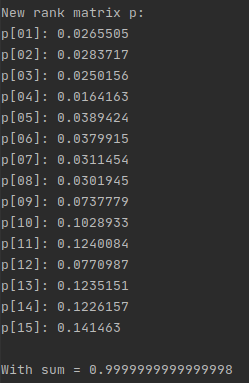
\includegraphics[width=150pt]{Exercise4/run_e.png}\\
\end{center}

Επομένως έχουμε διάνυσμα με τάξεις σελίδων:\\
\[\textbf{{\lt p}}=
    \left[ \begin{array}{c}
    0.0265505 \\
    0.0283717 \\
    0.0250156 \\
    0.0164163 \\
    0.0389424 \\
    0.0379915 \\
    0.0311454 \\
    0.0301945 \\
    0.0737779 \\
    0.1028933 \\
    0.1240084 \\
    0.0770987 \\
    0.1235151 \\
    0.1226157 \\
    0.141463 \\
    \end{array} \right]
\]

Απο το παραπάνω, παρατηρούμε ότι η τάξη της σελίδας 11 είναι 0.1240084 και της 10 είναι 0.1028933. Πρίν την αλλαγή η σελίδα 11 είχε τάξη 0.10632 και η 10 τάξη 0.10362. Επομένως, μπορούμε να συμπεράνουμε ότι η σελίδα 11 πέτυχε τον στόχο της και αύξησε την τάξη της κατά $0.1240084 - 0.10632 = 0.0176884$ ενω ο ανταγωνιστής της, η σελίδα 10, παρατήρησε μείωση: $0.1028933 - 0.10632 = -0.0034267$.

\section*{Ζητούμενο 6: Αποτέλεσμα διαγραφής της σελίδας 10}
Ζητείται να μελετηθεί επίδραση της διαγραφής της σελίδας 10 από το γράφημα.\\
Σε αυτή την περίπτωση αφαιρείται η 10η γραμμή και 10η στήλη του αρχικού πίνακα γειτνίασης. Επομένως, ο τροποποιημένος πίνακας γειτνίασης θα είναι ο:\\
\[\textbf{{\lt A}}=
    \left[ \begin{array}{cccccccccccccc}
    0 & 1 & 0 & 0 & 0 & 0 & 0 & 0 & 1 & 0 & 0 & 0 & 0 & 0 \\
    0 & 0 & 1 & 0 & 1 & 0 & 1 & 0 & 0 & 0 & 0 & 0 & 0 & 0 \\
    0 & 1 & 0 & 0 & 0 & 1 & 0 & 1 & 0 & 0 & 0 & 0 & 0 & 0 \\
    0 & 0 & 1 & 0 & 0 & 0 & 0 & 0 & 0 & 0 & 1 & 0 & 0 & 0 \\
    1 & 0 & 0 & 0 & 0 & 0 & 0 & 0 & 0 & 0 & 0 & 0 & 0 & 0 \\
    0 & 0 & 0 & 0 & 0 & 0 & 0 & 0 & 0 & 1 & 0 & 0 & 0 & 0 \\
    0 & 0 & 0 & 0 & 0 & 0 & 0 & 0 & 0 & 1 & 0 & 0 & 0 & 0 \\
    0 & 0 & 0 & 1 & 0 & 0 & 0 & 0 & 0 & 1 & 0 & 0 & 0 & 0 \\
    0 & 0 & 0 & 0 & 1 & 1 & 0 & 0 & 0 & 0 & 0 & 0 & 0 & 0 \\
    0 & 0 & 0 & 0 & 0 & 0 & 0 & 0 & 0 & 0 & 0 & 0 & 0 & 1 \\
    0 & 0 & 0 & 0 & 0 & 0 & 1 & 1 & 0 & 1 & 0 & 0 & 0 & 0 \\
    0 & 0 & 0 & 0 & 0 & 0 & 0 & 0 & 1 & 0 & 0 & 0 & 1 & 0 \\
    0 & 0 & 0 & 0 & 0 & 0 & 0 & 0 & 0 & 1 & 0 & 1 & 0 & 1 \\
    0 & 0 & 0 & 0 & 0 & 0 & 0 & 0 & 0 & 0 & 1 & 0 & 1 & 0 
    \end{array} \right]
\]

Το ζητούμενο υλοποιείται προγραμματιστικά στην γλώσσα {\lt python} στο αρχείο {\lt f\textunderscore 10\textunderscore deleted.py}  το οποίο φαίνεται παρακάτω:\\


\lt
\lstinputlisting[language=Python]{f_10_deleted.py}
\gt

Στον παραπάνω κώδικα:\\
Αρχικά, ορίζονται εκ νέου οι  συναρτήσεις {\lt construct\textunderscore G}, {\lt matrix\textunderscore columnMatrix\textunderscore multiplication}, {\lt integer\textunderscore columnMatrix\textunderscore multiplication} και {\lt power\textunderscore method} του αρχείου {\lt b\textunderscore G\textunderscore p\textunderscore calculation.py} που βρίσκεται στον ίδιο φάκελο {\lt Exercise4} μαζί με το τρέχον.
Αμέσως μετά βρίσκεται ο εκτελέσιμος κώδικας που θα εκτελεστεί αν εκτελέσουμε το αρχείο:\\
Ορίζεται ο πίνακας (γειτνίασης του γραφήματος) Α που είναι πανομοιότυπος με εκείνον του ζητούμενου 2 με εξαίρεση το ότι λείπει η γραμμή και στήλη 10.\\
Μετά, ορίζεται η μεταβλητή {\lt q} που αποθηκεύει την πιθανότητας μεταπήδησης (που έχει οριστεί απο την εκφώνηση σε 0.15) και η μεταβλητή {\lt n} που αποθηκεύει το μέγεθος του πίνακα Α. Στην συνέχεια, κατασκευάζεται ο πίνακας {\lt G}. Στην συνέχεια, υπολογίζεται το ιδιοδιάνυσμα της μέγιστης ιδιοτιμής (1) και αφού κανονικοποιηθεί αποτελεί τον πίνακα με τις τάξεις των σελίδων. Τέλος εμφανίζονται στην οθόνη οι τάξεις των σελίδων (στρογγυλοποιημένες σε 7 δεκαδικά ψηφία) και το άθροισμα όλων των τάξεων (για επαλήθευση ότι αθροίζουν στο 1 ως πιθανότητες).\\

Άν εκτελέσουμε το αρχείο αυτό το αρχείο θα δούμε στην οθόνη:\\
\begin{center}
    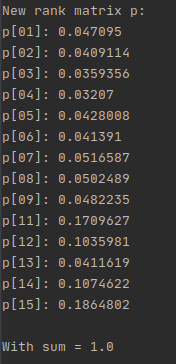
\includegraphics[width=150pt]{Exercise4/run_f.png}\\
\end{center}

(σημείωση: οι δείκτες {\lt i} του {\lt p[i]} που εμφανίζονται στο παραπάνω στιγμιότυπο και στο αποτέλεσμα εκτέλεσης του αρχείου αντιστοιχούν σε αρίθμηση σελιδών (στοιχεία του γραφήματος) και όχι θέση στο διάνυσμα με τάξεις)

Επομένως έχουμε διάνυσμα με τάξεις σελίδων:\\
\[\textbf{{\lt p}}=
    \left[ \begin{array}{c}
    0.047095 \\
    0.0409114 \\
    0.0359356 \\
    0.03207 \\
    0.0428008 \\
    0.041391 \\
    0.0516587 \\
    0.0502489 \\
    0.0482235 \\
    0.1709627 \\
    0.1035981 \\
    0.0411619 \\
    0.1074622 \\
    0.1864802 \\
    \end{array} \right]
\]

Απο τα παραπάνω αποτελέσματα παρατηρούμε ότι για τάξεις των σελιδών (σε σχέση με αυτές που πήραμε ως αποτέλεσμα στο ζητούμενο 2) ισχύει ότι οι τάξεις των σελιδών 9, 13 και 14 μειώνονται ενώ αυξάνονται οι τάξεις όλων των υπολοίπων σελιδών.
\end{document}
